\documentclass[a4paper,11pt]{kth-mag}
\usepackage[T1]{fontenc}
\usepackage{textcomp}
\usepackage{lmodern}
\usepackage[latin1]{inputenc}
\usepackage[swedish,english]{babel}
\usepackage{modifications}
\usepackage{amsmath}
\usepackage{amsthm}
\usepackage{amssymb}
\usepackage{amsfonts}
\usepackage{hyperref}
\usepackage{graphicx}
\usepackage{enumitem}
\usepackage{float}

\newcommand{\NN}{\ensuremath{\mathbb{N}}}
\newcommand{\ZZ}{\ensuremath{\mathbb{Z}}}
\newcommand{\QQ}{\ensuremath{\mathbb{Q}}}
\newcommand{\RR}{\ensuremath{\mathbb{R}}}
\newcommand{\CC}{\ensuremath{\mathbb{C}}}
\newcommand{\GG}{\ensuremath{\mathcal{G}}}

\newcommand{\Cpp}{\texttt{C++}}
\newcommand{\Gcc}{\texttt{gcc}}
\newcommand{\Gtkmm}{\texttt{gtkmm}}
\newcommand{\Gtk}{\texttt{GTK+}}
\newcommand{\Cairo}{\texttt{Cairo}}

\title{SimpleGraphPlotter v1.6}

\subtitle{Programkonstruktion f\"{o}r F, DD1342\\ Laboration 4A}
\foreigntitle{}
\author{Jim Holmstr\"{o}m\\\href{mailto:jimho@kth.se}{jimho@kth.se}}
\date{\today}
\blurb{Teacher: Ann Bengtson}

\trita{}
\begin{document}
\frontmatter
\pagestyle{empty}
\removepagenumbers
\maketitle
\selectlanguage{english}
\tableofcontents*
\mainmatter
\pagestyle{newchap}

\chapter{Introduction}
In the following part firstly the problem will be explained and secondly 
the requirements for a basic plotter will be listed.
A plotter is a program that can plot functions from strings which defines the 
functions by ordinary math syntax. 
The project uses \Cpp~ programming language and the 
\Gtkmm\footnote{Documentation, binaries and source can be found at: 
\href{http://www.gtkmm.org}{www.gtkmm.org}} wrapper for the 
\Gtk\footnote{Documentation, binaries and source can be found at: 
\href{http://www.gtk.org}{www.gtk.org}} toolkit to generate the graphical user interface.
Also \Cairo
\footnote{Documentation, binaries and source can be found at:
\href{http://www.cairographics.org/}{www.cairographics.org}
}
is used for the raw-rendering.\
It is compiled with the GNU \texttt{gcc-4.6.1} compiler and the repository for
the project can be found at
\href{
    https://github.com/Jim-Holmstroem/SimpleGraphPlotter
}{
    github.com/Jim-Holmstroem/SimpleGraphPlotter
} and are available under the GNU GPL license.

\section{Requirements}
\label{sec:requirements}
A few basic things is needed to have a functioning math plotter:
\begin{enumerate}
\item Define a function given ordinary math syntax.
\item Parse the inputed function and plot it accordingly.
\item Add/Remove functions from plotarea.
\item Plotarea should be scrollable both vertical and horizontal.
\item Range should be fixed to the unit-cube.\footnote{This restriction will be handled in section \ref{sec:scope}}
\item Display axis of the plot.
\item Parser must be properly tested.
\end{enumerate}

\section{Scope}
\label{sec:scope}
The functionality that is possible to put in a system like this is
almost endless so a few delimitations has to be made in order to complete the project.
The currently biggest restriction to the plotter is the lack of 
ability to zoom or change the range from the unit-cube.
No support for neither parametric nor complex functions.\footnote{
Since no native support in \Cpp~ for complex numbers which means 
all the basic math functions would have to be rewritten in order for this to work.}
Also no fileIO support.
\section{Assistance}
Besides the reference manuals for \Cairo, \Gtkmm~ and \Cpp~, no external help for 
this project was received.

\section{Compile and Run}
To code has been tested to be compiled and executed with Ubuntu 11.10. 
The program has one non-trivial dependency \Gtkmm\texttt{-3.0} which can be
installed from the package manager Synaptic under 
\texttt{libgtkmm-3.0-dev} (compile) 
and
\texttt{libgtkmm-3.0-1} (run).
\subsection{Compile}
Under the folder \texttt{/src} run
\begin{equation*}
   \texttt{make} 
\end{equation*}
The parser can also be compiled individually by under the folder
\texttt{/src/parser} run 
\begin{equation*}
   \texttt{make} 
\end{equation*}
\subsection{Run}
To run the program 
\begin{equation*}
   \texttt{./simplegraphplotter} 
\end{equation*}
The parser can also be executed individually by 
\begin{equation*}
    \texttt{./parser/parser\_test "-(x+sin(1+x))" 2}
\end{equation*}

\chapter{Structure}
A basic overview of the structure can be seen in figure \ref{fig:UML}, all
public non-self-explanatory parts will then be listed and explained in 
a \verb+javadoc+ like manner. In the actual code the definition and
implementation was separated into \texttt{.h} and \texttt{.cpp}-files
respectively as far as possible,\footnote{Some small trivial methods where
left out from this distinction as well as a few things that is hard or
impossible to separate in \Cpp.} and the code mostly follows Google's
style guide for \Cpp.\footnote{The style guide can be found at:
\href{
    http://google-styleguide.googlecode.com/svn/trunk/cppguide.xml
    }{
    google-styleguide.googlecode.com
    }
} 
The main goal of the structure for this project is to have as flexible code as possible.
\begin{figure}[H]
\begin{center}
    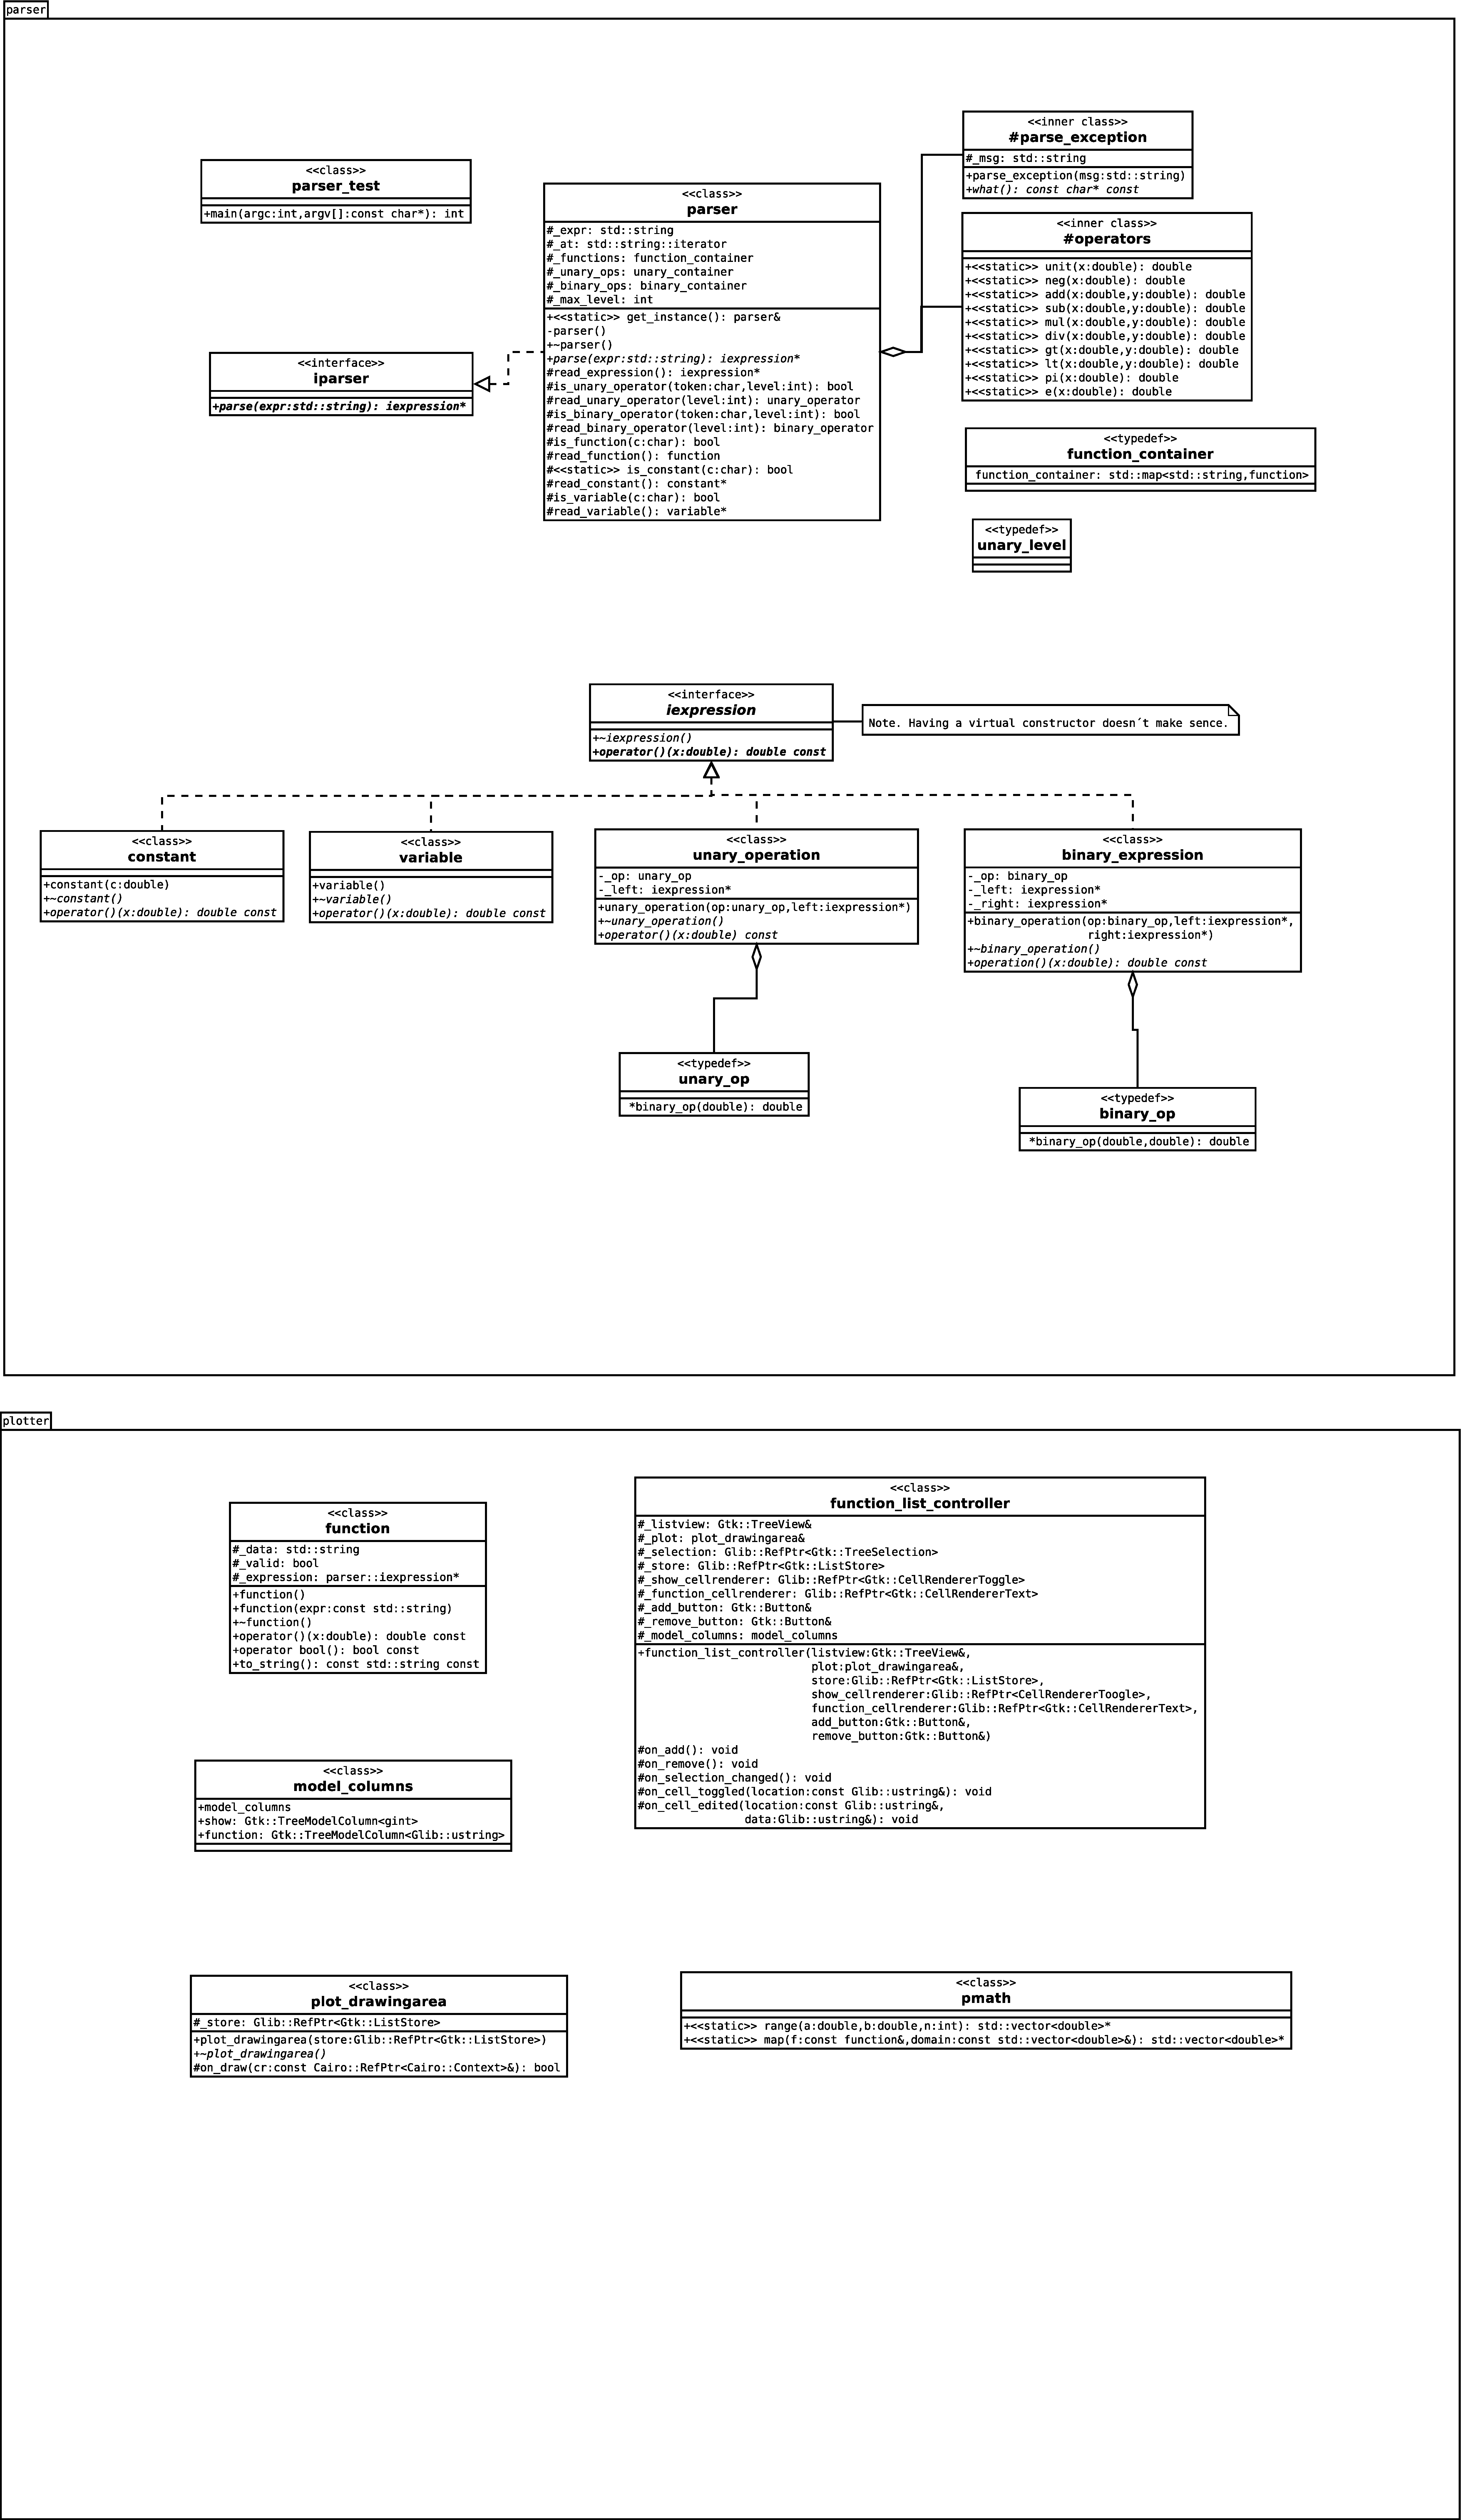
\includegraphics[width=0.8\textwidth]{uml.pdf}
    \caption{\small{An UML showing the structure and the enclosure.}}\label{fig:UML}
\end{center}
\end{figure}

\section{Parser}
The parser can be divided into two parts; the algorithm and the \emph{parse
tree} data structure. 

\begin{figure}[H]
\begin{center}
    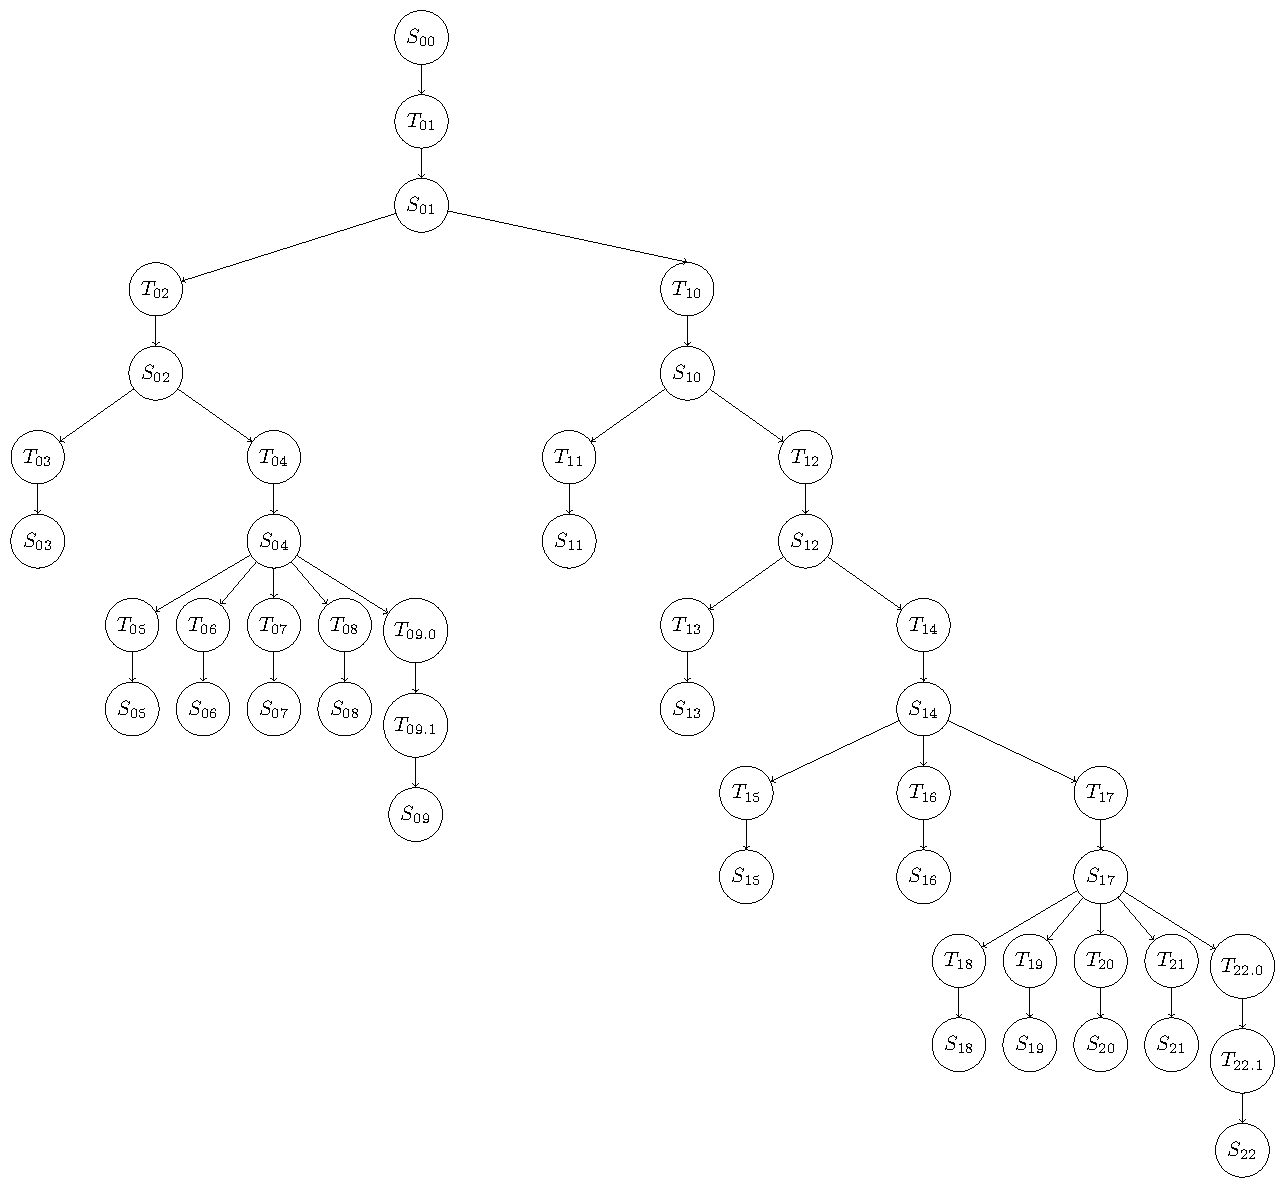
\includegraphics[width=0.5\textwidth]{parse-tree.pdf}
    \caption{\small{
        An example of the parse tree data structure generated by the parser
        from the expression \texttt{sin(x+2)*(x-1)}\texttt{\^~}\!\!\texttt{5}.
        Trivial nodes made by the actual implementation where
        here left out for added clarity.
    }}
   \label{fig:parsetree}
\end{center}
\end{figure}

\subsection{interface iparser}
An \emph{abstract base class} (ABC) that defines the \emph{interface} for what a parser 
needs to have to be considered a parser, this in case we want to compare 
different parser implementations or such.
\begin{description}
    \item[public parse(expr : std::string)] Virtual method which handles
    parsing the string \texttt{expr} to generate a parse tree that 
    represents the math expression in \texttt{expr}.
    \begin{description}
        \item[Parameters:]~\\
            \verb+expr+ - The string to be parsed.
        \item[Returns:]~\\
            A pointer to the root of the parse tree.
    \end{description}
\end{description}

\subsection{class parser}
The parser is a \emph{singelton} \emph{realization} of \texttt{iparser}
implementing a \emph{recursive descent parser} algorithm. Two
types of methods are used in the parsing, \texttt{is-a}\footnote{Starts with
\texttt{is\_}} and \texttt{read-it}\footnote{Starts with \texttt{read\_}}.
The \texttt{is-a} is used for look-ahead to determine the type of the expression
laying ahead, while \texttt{read-it} is used to do the actual syntactic 
information gathering from the expression fragment.
The EBNF\footnote{\href{www.cl.cam.ac.uk/~mgk25/iso-14977.pdf}{iso-14977.pdf}}
syntax for the parsing:\\
\begin{verbatim}
    plots  = term-(-1),[';',expression-(-1)],'\n' (* no support for ';' this \\
    implementation *) (* -1 is the lowest order expression *)
    expression-i = [unary-i],expression-(i+1),[op-(i+1),expression-i]
    term-n = var | num | [function],(,term-(-1),) \\
    (* n is the number of the highest order operator *)

    op-0 = '>' | '<'
    op-1 = '+' | '-'
    op-2 = '*' | '/' | '%'
    op-3 = '^'
    unary-3 = '+' | '-' | '*' 
    num = ? all numbers ?
    var = 'x'
    function = cos | sin | tan | acos | asin | atan | cosh \\
    | sinh | tanh | exp | log | log10 | sqrt | ceil | abs \\
    | floor | pi | e (* where pi and e are constant
    functions *)
\end{verbatim}
In the definition of \texttt{expression-i} either \texttt{unary-(i+1)} or
\texttt{op-(i+1)} is choosen. Unary, since on the left, has higher priority.


Worth noting is that the parser has two protected temporary instance variables
\texttt{\_expr}
and
\texttt{\_at} 
which are much more non-local than is needed. This might as well have 
been solved by passing them by reference down in the
parsing to preserve the locality to within the \texttt{parse} method. In favour
of code readability the later alternative was not considered.
This has the consequence that it makes some of the parsing 
methods technically non-\emph{static}, although the parser as a singelton can
therefore only have one instance per program in the same way as if it where static.

\begin{description}
    \item[static public get\_instance()]~\\
    Gets the singelton instance of the parser, if not yet instantiated it calls
    the private constructor and instantiates it.
    \begin{description}
        \item[Parameters:]~\\
            \verb+None+
        \item[Returns:]~\\
            A pointer to the singelton instance of the parser.
    \end{description}
\end{description}

\begin{description}
    \item[public parse(expr : std::string)] Parses the string \texttt{expr} to
    generate a parse tree that represents the math expression in \texttt{expr}.
    \begin{description}
        \item[Parameters:]~\\
            \verb+expr+ - The string to be parsed.
        \item[Returns:]~\\
            A pointer to the root of the parse tree.
    \end{description}
\end{description}

\subsection{interface iexpression}
\label{sec:iexpression}
Acts as abstract base class (ABC) for a node in the parse
tree, as the nodes in figure \ref{fig:parsetree}. The
\texttt{iexpression} is considered a \emph{functor} since it has overloaded the
\texttt{operator} and can thus be called as function.
The \texttt{operator} can be both 
\emph{recursively} implemented, as in
    \texttt{unary}\footnote{As can be seen in equation \ref{eq:unarydefined}.} 
    and
    \texttt{binary}\footnote{As can be seen in equation \ref{eq:binarydefined}.}, or
\emph{explicitly}\footnote{Explicit in the mathematical sense not as the keyword
in \Cpp.} implemented, as in 
    \texttt{constant}\footnote{As can be seen in equation \ref{eq:constantdefined}.} 
    and
    \texttt{variable}\footnote{As can be seen in equation \ref{eq:variabledefined}.}.
The operator function is generally defined by:
\begin{eqnarray}
    \label{eq:expressiondefined}
    \texttt{expression}: \RR &\rightarrow& \RR \nonumber \\
    x &\mapsto& \texttt{operator(}x\texttt{)} .
\end{eqnarray}

\begin{description}
    \item[public operator(x : double) double const] 
    Virtual definition of the \emph{evaluation} function for expressions. 
    Since the operator is going to act as a mathematical function one must be certain
    that it behaves like one, that is it does not modifies the functor when
    called.\footnote{In contrast to a method where that behaviour is allowed.}
    Therefore the \texttt{const} keyword has been added to prevent this
    from accidentally happening in the realizations.
    \begin{description}
        \item[Parameters:]~\\
            \verb+x+ - Input value for the expression. 
        \item[Returns:]~\\
            The output value of this expression given the parameter \texttt{x}.
    \end{description}
\end{description}

\subsection{class constant} A \emph{realization} of \texttt{iexpression}
\ref{sec:iexpression} which represents a constant. To keep constancy with the
iexpression this is implemented as a constant-function:
\begin{eqnarray}
    \label{eq:constantdefined}
    \texttt{constant}: \RR &\rightarrow& \RR \nonumber \\
    x &\mapsto& c .
\end{eqnarray}
\begin{description}
    \item[public constant(c : double)] Constructor 
    that constructs the function in the equation \ref{eq:constantdefined}. 
    \begin{description}
        \item[Parameters:]~\\
            \verb+c+ - The value of the constant in the expression.
    \end{description}
\end{description}
\begin{description}
    \item[public operator(x : double) double const] 
    Explicit realization of \texttt{iexpression.operator} returning a
    constant.
    \begin{description}
        \item[Parameters:]~\\
            \verb+x+ - Input value of the expression, does not matter only
            there for compatibility reasons. 
        \item[Returns:]~\\
            The output value of the expression.
    \end{description}
\end{description}

\subsection{class variable} A realization of \texttt{iexpression}
\ref{sec:iexpression} which represents a variable. A variable can simply be
seen as an unit-function:
\begin{eqnarray}
    \label{eq:variabledefined}
    \texttt{variable}: \RR &\rightarrow& \RR \nonumber \\
    x &\mapsto& x .
\end{eqnarray}
\begin{description}
    \item[public variable()] Constructor 
    that constructs the function in the equation \ref{eq:variabledefined}. 
    \begin{description}
        \item[parameters:]~\\
            \verb+None+
    \end{description}
\end{description}
\begin{description}
    \item[public operator(x : double) double const] 
    Explicit realization of \texttt{iexpression.operator} returning the value
    of the input.
    \begin{description}
        \item[Parameters:]~\\
            \verb+x+ - Input value of the expression.
        \item[Returns:]~\\
            The output value of the expression.
    \end{description}
\end{description}


\subsection{class unary\_operation} A realization of \texttt{iexpression}
\ref{sec:iexpression} which represents an unary operation, a function
constructed with \texttt{op} \texttt{left}:
\begin{eqnarray}
    \label{eq:unarydefined}
    \texttt{unary}:\RR &\rightarrow& \RR \nonumber \\
    x &\mapsto& \texttt{op(left(}x\texttt{))}. 
\end{eqnarray}

\begin{description}
    \item[public unary\_operation(op : unary\_op, left : iexpression*)] Constructor 
    that constructs the function in the equation \ref{eq:unarydefined}. 
    \begin{description}
        \item[Parameters:]~\\
            \verb+op+ - The unary operation performed, which is an \texttt{unary\_op}\footnote{Typedefined to
            be a function pointer: \texttt{*unary\_op(double):double}.}.\\
            \verb+left+ - The inner expression on which to perform the
            operation on.
    \end{description}
\end{description}
\begin{description}
    \item[public operator(x : double) double const] 
    Recursive realization of \texttt{iexpression.operator} returning the
    returned value of \texttt{left} through \texttt{op}, as in equation
    \ref{eq:unarydefined}.
    \begin{description}
        \item[Parameters:]~\\
            \verb+x+ - Input value for the \texttt{left} expression.
        \item[Returns:]~\\
            The returned value from the equation \ref{eq:unarydefined}.
    \end{description}
\end{description}

\subsection{class binary\_operation} A realization of \texttt{iexpression}
\ref{sec:iexpression} which represents a binary operation, that is a function
constructed with \texttt{op} and \texttt{left/right}:
\begin{eqnarray}
    \label{eq:binarydefined}
    \texttt{binary}: \RR &\rightarrow& \RR \nonumber \\
    x &\mapsto& \texttt{op(left(}x\texttt{),right(}x\texttt{))}.
\end{eqnarray}
\begin{description}
    \item[public binary\_operation(op : binary\_op, left : iexpression*, right :
    iexpression*)] Constructor that constructs the function in the equation
    \ref{eq:binarydefined}. 
    \begin{description}
        \item[Parameters:]~\\
            \verb+op+ - The unary operation performed, which is a
            \texttt{binary\_op}\footnote{Typedefined to
            be a function pointer: \texttt{*binary\_op(double,double):double}.}.\\
            \verb+left+ - The left expression on which to perform the
            operation on. \\
            \verb+right+ - The right expression on which to perform the
            operation on.
    \end{description}
\end{description}
\begin{description}
    \item[public operator(x : double) double const] 
    Recursive realization of \texttt{iexpression.operator} returning the
    returned values of \texttt{left} and \texttt{right} through \texttt{op},
    as in equation \ref{eq:binarydefined}.
    \begin{description}
        \item[Parameters:]~\\
            \verb+x+ - Input value for the expression.
        \item[Returns:]~\\
            The returned value from the equation \ref{eq:binarydefined}.
    \end{description}
\end{description}

\section{Plotter}
The GUI code for the plotter is coarsely separated into a \emph{MVC} pattern. 
The model in this project is the liststore for the \texttt{function}'s. This model 
has two different views: \texttt{Gtk::TreeView} which lists the functions, as can be seen
in figure \ref{fig:screenshotfunctionlistcontroller} and
\texttt{plot\_drawingarea}, as can be seen in figure
\ref{fig:screenshotplotarea}.
The controller is the \texttt{function\_list\_controller} which handles the
changes in the model and redraws the views when needed.
Almost all layout is separately define in an \texttt{.ui}-file\footnote{Follows XML
standard.} which is loaded by the \emph{builder} \texttt{Gtk::Builder} at startup.

\begin{figure}[H]
\begin{center}
    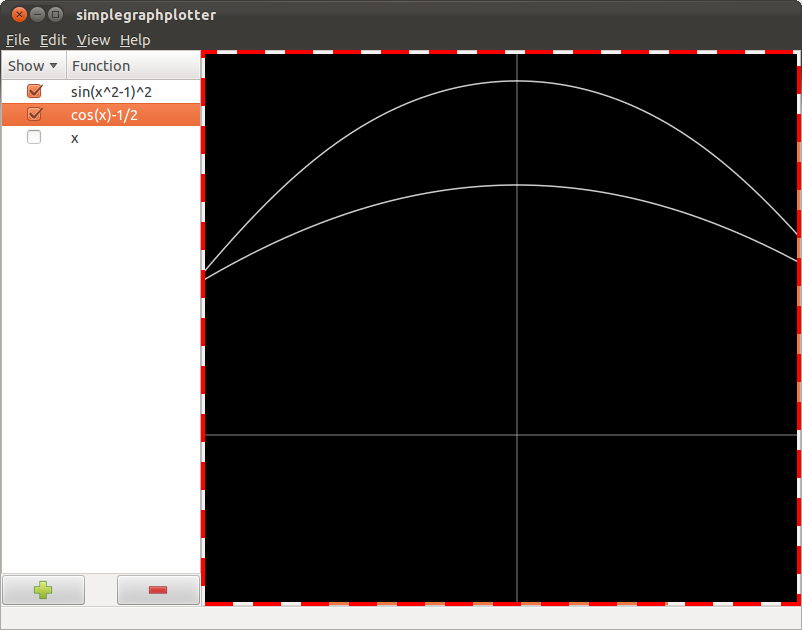
\includegraphics[width=0.7\textwidth]{screenshot00_plotarea.png}
    \caption{\small{A screenshot of the program under normal operation, with
    the plotarea highlighted.}}
   \label{fig:screenshotplotarea}
\end{center}
\end{figure}
\begin{figure}[H]
\begin{center}
    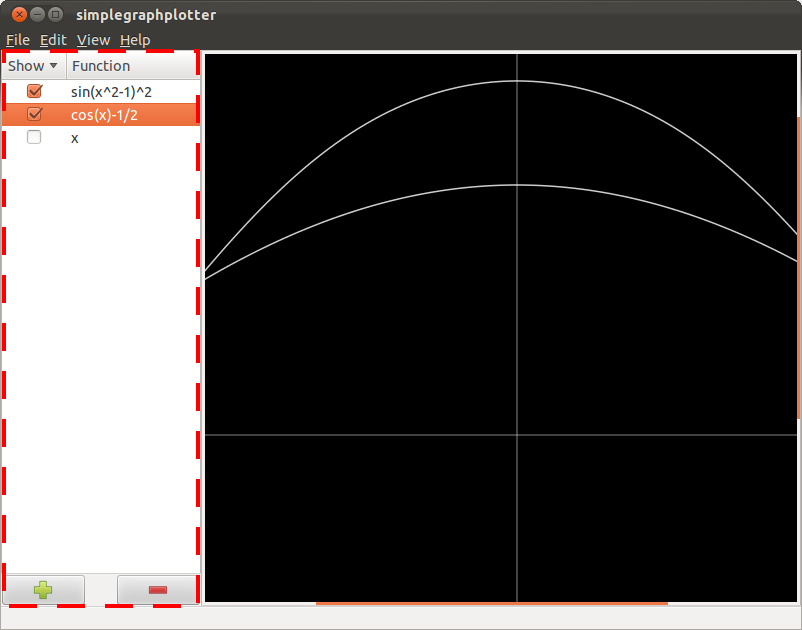
\includegraphics[width=0.7\textwidth]{screenshot00_function_list_controller.png}
    \caption{\small{A screenshot of the program under normal operation, with
    the treeview and add/remove buttons highlighted.}}
   \label{fig:screenshotfunctionlistcontroller}
\end{center}
\end{figure}

\subsection{class function}
Acts as a model of a function which is used by \texttt{plot\_drawingarea}.
It has the \emph{signature} for \texttt{iexpression} but it has not got the
same intended usage and should therefore not be a realization of
\texttt{iexpression}.

\begin{description}
    \item[public function(expr : const std::string)] Constructor 
    that constructs the function from the string \texttt{expr}.
    \begin{description}
        \item[Parameters:]~\\
            \verb+expr+ - The expression to use as a function.
    \end{description}
\end{description}

\subsection{class plot\_drawingarea}
Acts as a plotting view for the functions in the liststore \texttt{store}
provided in the constructor. It inherits from the \texttt{Gtk::DrawingArea} to
get some code and to have the right signature to work in the layout.

\begin{description}
    \item[public plot\_drawingarea(store : Glib::RefPtr<Gtk::ListStore>)] Constructor 
    that constructs a \texttt{plot\_drawingarea}. 
    \begin{description}
        \item[Parameters:]~\\
            \verb+store+ - Reference\footnote{\texttt{Gtk::RefPtr} is an
            reference-counting shared smart pointer.} to the liststore that contains the
            functions to be rendered. Must be, or in the same format as
            \texttt{function\_store} defined in the \texttt{.ui}-file.
    \end{description}
\end{description}

\begin{description}
   \item[protected on\_draw(cr : const Cairo::RefPtr<Cairo::Context>\&)]~\\
   The draw signal handler for the \texttt{plot\_drawingarea}.
   \begin{description}
        \item[Parameters:]~\\
            \verb+cr+ - The reference to the \texttt{Cairo::Context} on which to draw on.
        \item[Returns:]~\\
            Mostly true.
    \end{description}
\end{description}

\subsection{class function\_list\_controller}
A \emph{controller} that handles the functions. The protected methods starting
with \texttt{on\_} is \emph{action listeners} and can be overriden in a
new child class to change the functionality on them without the need to
reimplement the basecode.\footnote{One should always avoid code duplication.}
\begin{description}
    \item[{
    \parbox[t]{\linewidth}
        {
        public function\_list\_controller(\\
            listview : Gtk::TreeView\&,\\
            plot : plot\_drawingarea\&,\\
            store : Glib::RefPtr<Gtk::ListStore>,\\ 
            show\_cellrenderer : Glib::RefPtr<Gtk::CellRendererText>,\\
            add\_button : Gtk::Button\&,\\
            remove\_button : Gtk::Button\&\\
            )
        }
    }]~\\
    Constructor for \texttt{function\_list\_controller}.
    \begin{description}
        \item[Parameters:]~\\
            \verb+listview+ - Reference to the view of the list.\\
            \verb+plot+ - Reference to the plot view for the functions.\\
            \verb+store+ - Reference to the liststore that handles the functions.\\
            \verb+show_cellrenderer+ - Reference to the
            \texttt{Gtk::CellRendererText} which defines the textfield's
            appearance in the \texttt{store}.\\
            \verb+add_button+ - A reference to the button that controls adding
            new functions into the \texttt{store}.\\
            \verb+remove_button+ - A reference to the button that controls
            removing functions from the \texttt{store}.
    \end{description}
\end{description}

\begin{description}
    \item[protected on\_add()]~\\
    Signal handler for adding a function.
    \begin{description}
        \item[Parameters:]~\\
            \verb+None+
    \end{description}
\end{description}
\begin{description}
    \item[protected on\_remove()]~\\
    Signal handler for removing a function.
    \begin{description}
        \item[Parameters:]~\\
            \verb+None+
    \end{description}
\end{description}
\begin{description}
    \item[protected on\_selection\_changed()]~\\
    Signal handler for selection change.
    \begin{description}
        \item[Parameters:]~\\
            \verb+None+
    \end{description}
\end{description}
\begin{description}
    \item[protected on\_cell\_toggled(location : const Glib::ustring\&)]~\\
    Signal handler for toggling the visibility of a function.
    \begin{description}
        \item[Parameters:]~\\
            \verb+location+ - The location in the liststore of the function
            being toggled.
    \end{description}
\end{description}
\begin{description}
    \item[protected on\_cell\_edited(location : const Glib::ustring\&, 
        data : const Glib::ustring\&)]~\\
    Signal handler for editing a function.
    \begin{description}
        \item[Parameters:]~\\
            \verb+location+ - The location in the liststore of the function
            begin edited. \\
            \verb+data+ - What the function is being edited to.
    \end{description}
\end{description}

\chapter{Results and Discussion}

\section{Results}
A screenshot of the final result of this project can be seen in figure
\ref{fig:screenshot}.
\begin{figure}[H]
\begin{center}
    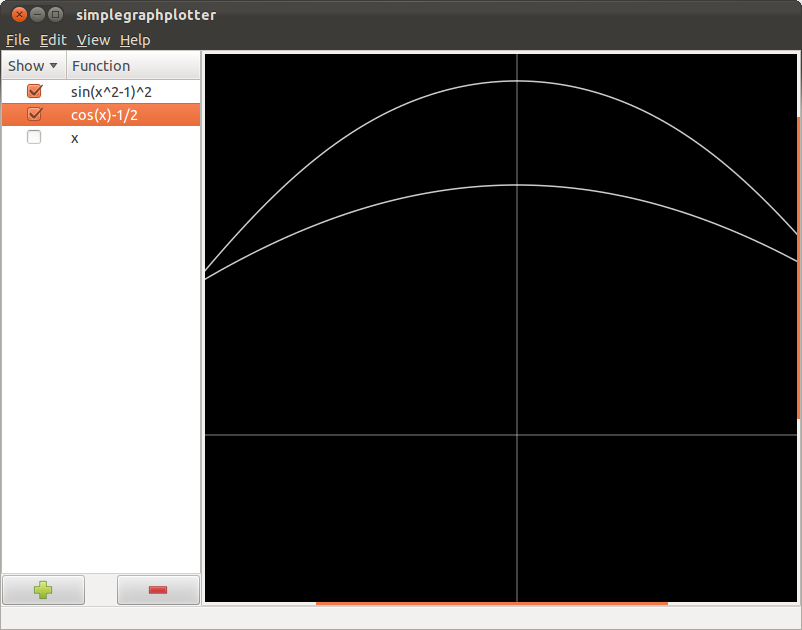
\includegraphics[width=0.75\textwidth]{screenshot00.png}
    \caption{\small{A screenshot of the program under normal operation.}}
   \label{fig:screenshot}
\end{center}
\end{figure}

The program did not have any memory leaks under normal operations when tested in the program
\texttt{valgrind}.

All the points in the list from section \ref{sec:requirements} was fulfilled
and no failing test cases for the parser was found. 

\section{Discussion}
    \subsection{Problems}
        The unofficial \Cpp wrapper 
        \Gtkmm\footnote{Which only was used to get inheritance, polymorphism
        and having it  compatible with the standard \Cpp Library.} where quite 
        immature and to implement much of the common functionality for this 
        type of applications easily became hacky or needed to workaround bugs. 
        Also the sparse documentation was sometimes a problem.
        
        In a parser it is easy to miss out test case combinations, the latest miss
        which almost went trough to release was a priority miss between
        unary and binary operators which resulted in:
        \begin{equation*}
            -x^2=(-x)^2
        \end{equation*}
        which is not the case for math expressions.

    \subsection{Reflections}
        One needs, even in this rather small project, quite a few iterations 
        of the overall design as well as on the lower level to get an overall good and flexible
        structure.

\end{document}
